%----------------------------------------------------------------------------------------
%	CLASS, PACKAGES AND OTHER DOCUMENT CONFIGURATIONS
%----------------------------------------------------------------------------------------

\documentclass[
	a4paper, % Paper size, use either a4paper or letterpaper
	12pt, % Default font size, the template is designed to look good at 12pt so it's best not to change this
	%unnumberedsections, % Uncomment for no section numbering
]{CSSullivanBusinessReport}
\usepackage{tikz}
\usetikzlibrary{arrows.meta,
                chains,
                positioning}
\usepackage{colortbl}
\usepackage{multirow}
\addbibresource{references.bib} % BibLaTeX bibliography file
\usepackage{caption}
\usepackage{subcaption}

%----------------------------------------------------------------------------------------
%	REPORT INFORMATION
%----------------------------------------------------------------------------------------

\reporttitle{CARE Lab Social Engineering Competition} % The report title to appear on the title page and page headers, do not create manual new lines here as this will carry over to page headers

\reportsubtitle{Day Two Deliverables} % Report subtitle, include new lines if needed

\reportauthors{Authors:\\\smallskip Liam Geyer (lfg5289@psu.edu)\\\smallskip Jenna Fox (jef5600@psu.edu)\\\smallskip Brendan McShane (bbm5360@psu.edu)\\\smallskip Jonathan Skeete (jxs7245@psu.edu)} % Report authors/group/department, include new lines if needed

\reportdate{April 20, 2024} % Report date, include new lines for additional information if needed

\rightheadercontent{\includegraphics[height=1.5cm]{assets/branding/ccso-shield.png}} % Header logo

%----------------------------------------------------------------------------------------

\begin{document}

%----------------------------------------------------------------------------------------
%	TEMPLATE PAGES
%----------------------------------------------------------------------------------------

\input{template/title-page.tex}
\begin{twothirdswidth} % Content in this environment to be at two-thirds of the whole page width
	\tableofcontents % Output the table of contents, automatically generated from the section commands used in the document
\end{twothirdswidth}

\newpage

%----------------------------------------------------------------------------------------
%	SECTIONS
%----------------------------------------------------------------------------------------

\begin{fullwidth}
\section{Executive Summary}

The CARE Lab Fraud Fighters Team continued efforts to assist Sam with her hiring process and determining the legitimacy of her offer. During the second day of the engagement, the team met with Sam to provide guidance throughout a text-based job interview conducted on Microsoft Teams. There were a number of red flags encountered during the interview as well as discrepancies between the information provided within the interview and the initial email. The most notable of these discrepancies was that Mr. David W. Bondeson did not conduct the interview as previously mentioned and that the company Omnicell, Inc was used interchangeably with HealthComp, LLC despite no relation.\\\medskip

Afterwards, the team sat in on a follow up text based meeting with Sam during which she received a job offer email from the prospective employer/scammer. This email contained several red flags potentially indicating it as a phishing email. As part of the on boarding process Sam was asked to fill out a job application form, W4, and provide a passport photo.\\\medskip

The team has compiled a comprehensive report detailing OSINT findings, potential red flags, a comprehensive timeline with MITRE ATT\&CK Mappings, NIST Phish Scale evaluations of Sam's emails, as well as a to-do list and game plan for Sam moving forward. The compiled evidence indicates that this employment opportunity is extremely likely to be a scam; the team has prepared a comprehensive brief to communicate the red flags, and risks of moving forward to Sam.
\end{fullwidth}
\begin{fullwidth}
\section{OSINT Findings} % Top level section
\subsection{BBB Scam Report}

The team found a report submitted to the Better Business Bureau which fits the exact description of Sam's interactions with the prospective employer.

\begin{quote}
	\textbf{\LARGE ``}I was sent an email about a potential job offer for HealthComp I then got instructions to conduct an interview on Microsoft Team then they so called hired me and had me fill out paper work including a W4 form that had my ssn number then after that I told them I had finished filling out the paper work and then they started asking if I was going to be using a credit card to accept my payments and I said no then they said I need one so they can process faster then that's when I realized it was a scam\textbf{''}
	
	\hfill--- BBB Scam ID \#772647 \autocite{BBB:2023}
\end{quote}

The BBB Scam Report lists the same davidbondeson@healthcomp.live email address referenced in Sam's interview offer. With this in mind, it's extremely likely that Sam's job opportunity is not legitimate.

\subsection{Employer Information}
    \begin{itemize}
        \item HealthComp signed a merger with Virgin Pulse to create Personify Health. Omnicell is not affiliated with HealthComp or Personify Health whatsoever.
    \\\medskip
        \item All positions offered to Sam are not posted on Personify Health's or Omnicell's internal job board \hyperref[sec:Fig1]{(See Figure 1)}.
    \\\medskip
    \end{itemize}

\subsection{Interviewer Information}
    \begin{itemize}
        \item As of Nov. 2023, Mr. Manley has left Omnicell, Inc. He is now employed as a Senior Enterprise Account Executive at Docusign, Inc. \hyperref[sec:Fig2]{(See Figure 2)}.
    \\\medskip
        \item Mr. Manley's LinkedIn profile indicates that he received a Bachelor of Science in Business Administration from the University of Central Florida \hyperref[sec:Fig3]{(See Figure 3)}.
    \\\medskip        
        \item During his time at Omnicell, Mr. Manley was a Medical Account Executive.
    \\\medskip        
        \item David W. Bondeson is not an Interview Manager but the Director of Stop Loss Sales \hyperref[sec:Fig4]{(See Figure 4)}.
    
    \end{itemize}

\subsection{Domain Information}
    \begin{itemize}
        \item Mr. David W. Bondeson should uses a healthcomp.com domain instead of healthcomp.live \hyperref[sec:Fig5]{(See Figure 5)}.
        \item The healtcomp.live domain was registered in 2023, whereas the healthcomp.com domain was registered in 2001 \hyperref[sec:Fig6]{(See Figure 6)}.
    \end{itemize}

\subsection{OSINT Evidence}
    \begin{figure*}[H] % Use the figure* environment for full width figures
        \label{sec:Fig1}
        \centering
        \includegraphics[width=.9\linewidth]{assets/realJobPosting.png}
        \captionsetup{justification=centering}
        \caption{The job listings for Healthcomp do not have the offered position of content writer available.}
    \end{figure*}
    
    \begin{figure*}[H] % Use the figure* environment for full width figures
        \label{sec:Fig2}
        \centering
        \includegraphics[width=.9\linewidth]{assets/ManleyLinkedin2.png}
        \captionsetup{justification=centering}
        \caption{Gavin Manley's LinkedIn profile showing his employment at Omnicell, Inc ended in November 2023 due to his transition to DocuSign as a Senior Enterprise Account Executive.}
    \end{figure*}

    \begin{figure*}[H] % Use the figure* environment for full width figures
        \label{sec:Fig3}
        \centering
        \includegraphics[width=.9\linewidth]{assets/ManleyCollege.png}
        \captionsetup{justification=centering}
        \caption{Gavin Manley's LinkedIn profile showing he graduated from the University of Central Florida.}
    \end{figure*}

    \begin{figure*}[H] % Use the figure* environment for full width figures
        \label{sec:Fig4}
        \centering
        \includegraphics[width=.9\linewidth]{assets/BondesonLinkedinHeader.png}
        \captionsetup{justification=centering}
        \caption{David W. Bondeson is listed as Director of Stop Loss Sales at Personify Health.}
    \end{figure*}

    \begin{figure*}[H] % Use the figure* environment for full width figures
        \label{sec:Fig5}
        \centering
        \includegraphics[width=.9\linewidth]{assets/bondeson-email.png}
        \captionsetup{justification=centering}
        \caption{David W. Bondeson's contact information on LinkedIn.}
    \end{figure*}

    \begin{figure*}[H] % Use the figure* environment for full width figures
        \label{sec:Fig6}
        \centering
        \begin{subfigure}{0.5\textwidth}
            \centering
            \includegraphics[width=1.37\linewidth]{assets/ICANN Lookup.png}
            \captionsetup{justification=centering}
            \caption{healthcomp.com Domain Registration (2001)}
        \end{subfigure}
        \hfill
        \begin{subfigure}{0.5\textwidth}
            \centering
            \includegraphics[width=1.37\linewidth]{assets/ICANN Lookup2.png}
            \captionsetup{justification=centering}
            \caption{healthcomp.live Domain Registration (2023)}
        \end{subfigure}
        \hfill
        \captionsetup{justification=centering}
        \caption{Two different domains for the same company}
    \end{figure*}

\end{fullwidth}
\begin{fullwidth}
\section{Red Flags} % Top level section
\begin{enumerate}
    \item \textbf{Potential AI Chat-bot}
            \\\medskip
                \item[--] The interviewer, who is claiming to be human, is responding in a time frame that is unrealistic to expect from a real person.
            \\\medskip
                \item[--] When texting Sam was asked for certain keywords which would serve as a prompt for the chat-bot to generate text tailored to their current conversation \hyperref[sec:Fig7]{(See Figure 7)}.
            \\\medskip
    \item \textbf{Inconsistent Information}
            \\\medskip
                \item[--] Neither Mr. Bondeson, Mr. Manly, or Ms. McDaniel ever refer to HealthComp by it's new name, Personify Health.
            \\\medskip
                \item[--] The original interview offer Sam received was from HealthComp, LLC. Upon entering the interview, it was revealed that she was actually interviewing for a company called Omnicell \hyperref[sec:Fig8]{(See Figure 8)}. After reviewing public records, the team concluded that Omnicell is not affiliated with HealthComp or Personify Health whatsoever.
            \\\medskip
                \item[--] In the beginning of the interview, Mr. Manley introduces himself to be from Omincell, Inc., but  later switches to HealthComp, LLC. \hyperref[sec:Fig9]{(See Figure 9)}.
            \\\medskip
                \item[--] The job offer letter Sam received was for HealthComp, which was consistent with the initial email, but not with the text based interview.
    \item \textbf{Point of Contact Discrepancies}
            \\\medskip
                \item[--] As stated in the email sent from HealthComp, LLC, the point of contact for this interview was supposed to be Mr. David W. Bondeson; however, the interviewer introduces himself as Mr. Gavin Manley from Omnicell, Inc. despite having the contact name "david donbenson" in Teams \hyperref[sec:Fig10]{(See Figure 10)}.
            \\\medskip
                \item[--] In the interview, Mr. Manley Introduces himself to be from Omnicell, Inc., but according to his Linkedin profile, he's currently employed at Docusign as a Senior Enterpise Account Executive \hyperref[sec:Fig2]{(See Figure 2)}.
            \\\medskip
                \item[--] When introducing himself, Mr. Manley states that he received his Bachelor of Science in Electrical Engineering from the Swiss University of Applied Science, Winterthur \hyperref[sec:Fig11]{(See Figure 11)}. This information is inconsistent with Mr. Manley’s LinkedIn profile indicates that he received a Bachelor of Science in Business Administration from the University of Central Florida \hyperref[sec:Fig3]{(See Figure 3)}.
            \\\medskip 
                \item[--] During his time at Omnicell, Mr. Manley was a Medical Account Executive and not on the board of directors as he claims in the interview \hyperref[sec:Fig2]{(See Figure 2)}. 
            \\\medskip
                \item[--] Mr. Bondeson's title at HealthComp, LLC. is Director of Stop Loss sales and not Interview Manager \hyperref[sec:Fig4]{(See Figure 4)}.
            \\\medskip
                \item[--] Kellie McDaniel is not listed as a HealthComp employee
            \\\medskip
                \item[--] Email requests all communication be sent through a @healthcomp.live domain instead of the official @healthcomp.com domain listed on their Linkedin and website \hyperref[sec:Fig5]{(See Figure 5)}.
    \item  \textbf{Professionalism}
            \\\medskip
                \item[--] Numerous grammar \hyperref[sec:Fig12]{(See Figures 12-13)}, spelling \hyperref[sec:Fig14]{(See Figure 14)}, and convention errors \hyperref[sec:Fig15]{(See Figure 15)}.
            \\\medskip
                \item[--] Does not address recipient of email in interview offer letter and instead refers to Sam as Candidate and uses a verification code to track her application \hyperref[sec:Fig14]{(See Figure 16)}.
            \\\medskip
                \item[--] Email signed by HealthComp instead of the sender or an HR Representative \hyperref[sec:Fig16]{(See Figure 16)}.
                \item[--] Lack of branding on throughout all contact, most companies will usually include a header, footer, and logo in their emails. 
            \\\medskip            
                \item[--] The contact name on the Microsoft Teams chat reads, "david donbenson" and not "David Bondeson," lacking proper capitalization and spelling of the last name provided in the original email \hyperref[sec:Fig17]{(See Figure 17}). 
    \item   \textbf{Lure}
            \\\medskip
                \item[--] Offer letter states Sam will have to purchase her own office equipment from a supplied vendor and will be reimbursed, which is a common scam acknowledged by the Federal Trade Commission. The vendor could be one the scammers created themselves to have payment redirected towards them, and you wont receive the products ordered 
                \item[--] Employer requests a photo of Sam, which could be used for identity theft 
\end{enumerate}

\subsubsection{Red Flag Evidence}
    \begin{figure*}[H] % Use the figure* environment for full width figures
        \label{sec:Fig7}
        \centering
        \includegraphics[width=.75\linewidth]{assets/chatbot.png}
        \captionsetup{justification=centering}
        \caption{The interviewer asked Sam to reply with "DONE" or other cue words at several points.}
    \end{figure*}

    \begin{figure*}[H] % Use the figure* environment for full width figures
        \label{sec:Fig8}
        \centering
        \begin{subfigure}{0.5\textwidth}
            \centering
            \includegraphics[width=1.37\linewidth]{assets/Healthcomp.png}
            \captionsetup{justification=centering}
            \caption{Initial Email from HealthComp, LLC.}
        \end{subfigure}
        \hfill
        \begin{subfigure}{0.5\textwidth}
            \centering
            \includegraphics[width=1.37\linewidth]{assets/Omnicell.png}
            \captionsetup{justification=centering}
            \caption{Interview introduction as Omnicell, Inc.}
        \end{subfigure}
        \hfill
        \captionsetup{justification=centering}
        \caption{Discrepancy in the company offering the job.}
    \end{figure*}

    \begin{figure*}[H] % Use the figure* environment for full width figures
        \label{sec:Fig9}
        \centering
        \begin{subfigure}{0.5\textwidth}
            \centering
            \includegraphics[width=1.37\linewidth]{assets/Omnicell.png}
            \captionsetup{justification=centering}
            \caption{Interview introduction as Omnicell, Inc.}
        \end{subfigure}
        \hfill
        \begin{subfigure}{0.5\textwidth}
            \centering
            \includegraphics[width=1.37\linewidth]{assets/switchToHealthcomp.png}
            \captionsetup{justification=centering}
            \caption{HealthComp used later in the interview.}
        \end{subfigure}
        \hfill
        \captionsetup{justification=centering}
        \caption{The interviewer switches between HealthComp and Omnicell.}
    \end{figure*}


    \begin{figure*}[H] % Use the figure* environment for full width figures
        \label{sec:Fig10}
        \centering
        \includegraphics[width=.75\linewidth]{assets/ManelyIntroduction.png}
        \captionsetup{justification=centering}
        \caption{The interviewer introduces himself as Mr. Gavin Manley.}
    \end{figure*}

    \begin{figure*}[H] % Use the figure* environment for full width figures
        \label{sec:Fig11}
        \centering
        \includegraphics[width=.9\linewidth]{assets/ManleyInterviewCollege.png}
        \captionsetup{justification=centering}
        \caption{Mr. Manley claimed to have graduated from the Swiss University of Applied Science.}
    \end{figure*}

    \begin{figure*}[H] % Use the figure* environment for full width figures
        \label{sec:Fig12}
        \centering
        \includegraphics[width=.9\linewidth]{assets/missedCommas.png}
        \captionsetup{justification=centering}
        \caption{There should be a comma following "\$27/hr" and before "but"}
    \end{figure*}

    \begin{figure*}[H] % Use the figure* environment for full width figures
        \label{sec:Fig13}
        \centering
        \includegraphics[width=.9\linewidth]{assets/runon.png}
        \captionsetup{justification=centering}
        \caption{This is a run-on sentence that should be broken up into two or three separate sentences.}
    \end{figure*}

    \begin{figure*}[H] % Use the figure* environment for full width figures
        \label{sec:Fig13}
        \centering
        \includegraphics[width=.9\linewidth]{assets/misspelling.png}
        \captionsetup{justification=centering}
        \caption{Misspelling of "fitment". It should just say "fit".}
    \end{figure*}

    \begin{figure*}[H] % Use the figure* environment for full width figures
        \label{sec:Fig14}
        \centering
        \includegraphics[width=.9\linewidth]{assets/titleerror.png}
        \captionsetup{justification=centering}
        \caption{Discrepancy between "Mr.David W. Bondeson" compared to "Mr David W. Bondeson".}
    \end{figure*}

    \begin{figure*}[H] % Use the figure* environment for full width figures
        \label{sec:Fig15}
        \centering
        \includegraphics[width=.9\linewidth]{assets/VerificationCode.png}
        \captionsetup{justification=centering}
        \caption{Verification code to be used as identification and email signature from HealthComp}
    \end{figure*}

    \begin{figure*}[H] % Use the figure* environment for full width figures
        \label{sec:Fig16}
        \centering
        \begin{subfigure}{0.5\textwidth}
            \centering
            \includegraphics[width=1.37\linewidth]{assets/BondesonEmail.png}
            \captionsetup{justification=centering}
            \caption{Original email with correct spelling.}
        \end{subfigure}
        \hfill
        \begin{subfigure}{0.5\textwidth}
            \centering
            \includegraphics[width=1.37\linewidth]{assets/TeamsNamepng.png}
            \captionsetup{justification=centering}
            \caption{Misspelled name in Microsoft Teams interview.}
        \end{subfigure}
        \hfill
        \captionsetup{justification=centering}
        \caption{There is a clear misspelling between the point of contact and the Teams account hosting the interview.}
    \end{figure*}

\end{fullwidth}
\begin{fullwidth}
\section{Timeline \& ATT\&CK Mappings} % Top level section

\subsection{Timeline}
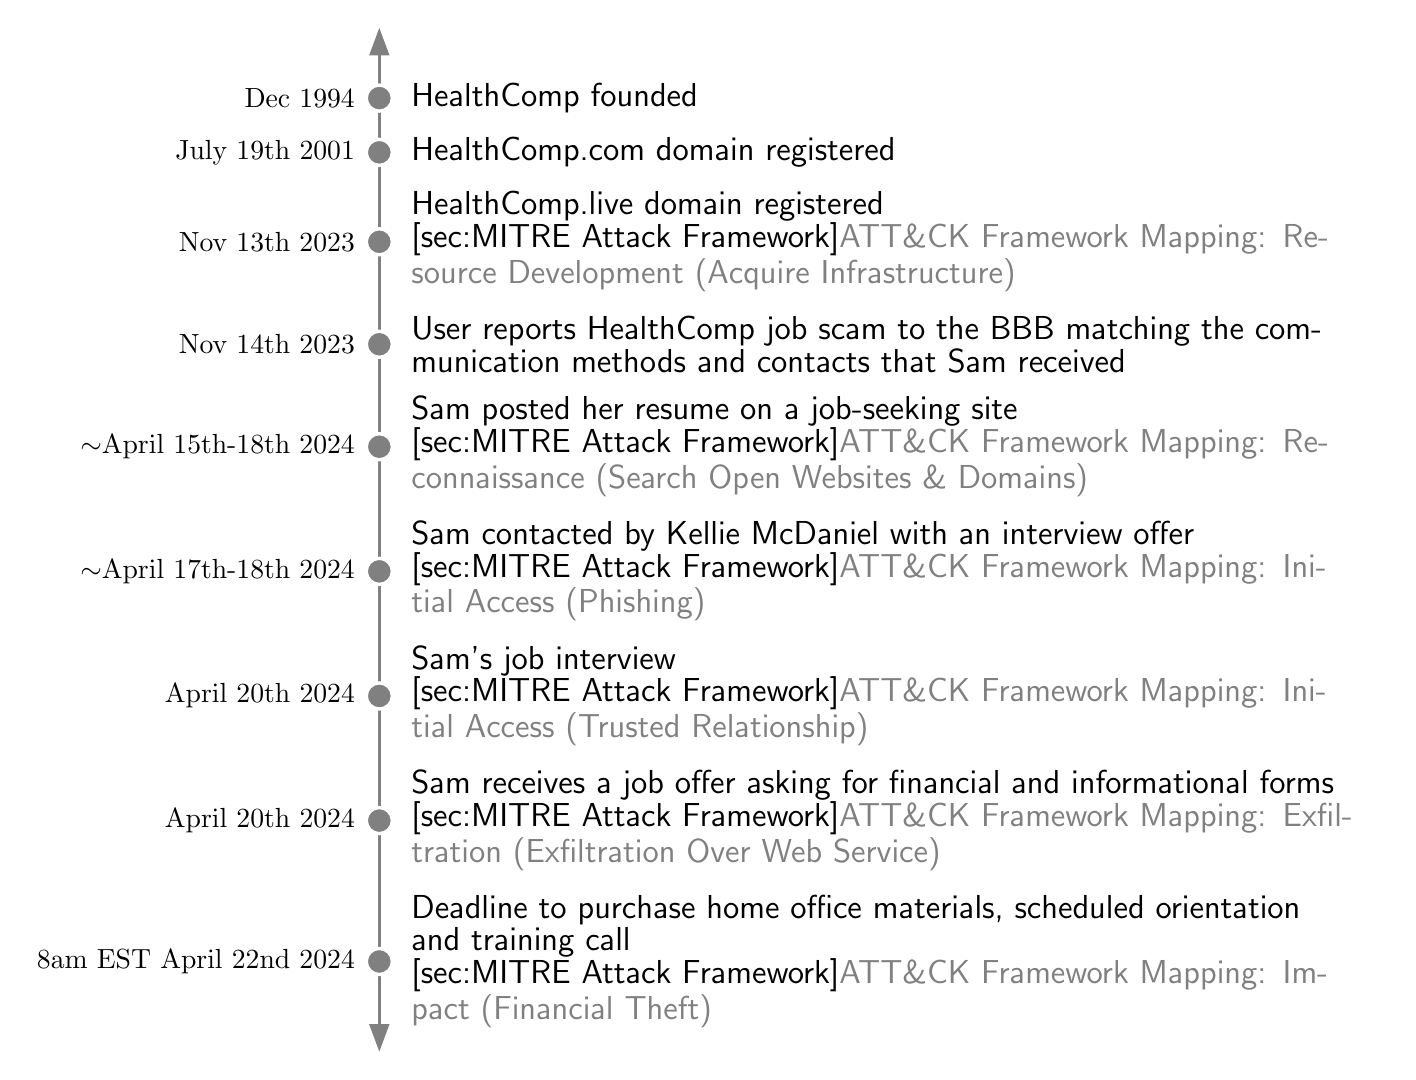
\begin{tikzpicture}[
node distance = 1mm and 3mm,
  start chain = A going below,
   dot/.style = {circle, draw=white, very thick, fill=gray,
                 minimum size=3mm},
   box/.style = {rectangle, text width=120mm,
                 inner xsep=4mm, inner ysep=1mm,
                 font=\sffamily\large\linespread{0.84}\selectfont,
                 on chain},
                        ]
    \begin{scope}[every node/.append style={box}]
    \node { HealthComp founded} ;
    \node { HealthComp.com domain registered} ;
    \node { HealthComp.live domain registered\\
    \hyperref[sec:MITRE Attack Framework]{\textcolor{gray}{ATT\&CK Framework Mapping: Resource Development (Acquire Infrastructure)}}} ;
    \node { User reports HealthComp job scam to the BBB matching the communication methods and contacts that Sam received} ;
    \node { Sam posted her resume on a job-seeking site\\
    \hyperref[sec:MITRE Attack Framework]{\textcolor{gray}{ATT\&CK Framework Mapping: Reconnaissance (Search Open Websites \& Domains)}}} ;
    \node { Sam contacted by Kellie McDaniel with an interview offer\\
    \hyperref[sec:MITRE Attack Framework]{\textcolor{gray}{ATT\&CK Framework Mapping: Initial Access (Phishing)}}} ;
    \node { Sam's job interview\\
    \hyperref[sec:MITRE Attack Framework]{\textcolor{gray}{ATT\&CK Framework Mapping: Initial Access (Trusted Relationship)}}} ;
    \node{ Sam receives a job offer asking for financial and informational forms\\
    \hyperref[sec:MITRE Attack Framework]{\textcolor{gray}{ATT\&CK Framework Mapping: Exfiltration (Exfiltration Over Web Service)}}} ;
    \node { Deadline to purchase home office materials, scheduled orientation and training call\\
    \hyperref[sec:MITRE Attack Framework]{\textcolor{gray}{ATT\&CK Framework Mapping: Impact (Financial Theft)}}} ;
    \end{scope}
\draw[very thick, gray, {Triangle[length=10pt)]}-{Triangle[length=10pt]}, % arrow size  
      shorten <=-6mm, shorten >=-2mm] % length of arrows
    (A-1.north west) -- (A-9.south west); % number of nodes in timeline
\foreach \i [ count=\j] in {Dec 1994, July 19th 2001, Nov 13th 2023, Nov 14th 2023, $\sim$April 15th-18th 2024, $\sim$April 17th-18th 2024, April 20th 2024, April 20th 2024, 8am EST April 22nd 2024}
    \node[dot,label=left:\i] at (A-\j.west) {};
    \end{tikzpicture}

\subsection{MITRE ATT\&CK Framework Mappings}

\begin{enumerate}
    \item \textbf{Resource Development: Acquire Infrastructure T1583}
        \\\medskip On Nov 13, 2023 the healthcomp.live domain is registered for use in later scams and phishing campaigns. This maps closely with the first reported HealthComp scam which was reported the next day.
    \item \textbf{Reconnaissance: Search Open Websites \& Domains T1593}
        \\\medskip Sam posted her resume to a public job-seeking site somewhere between April 15-18, 2024. She was contacted shortly offer with the interview offer from Kellie McDaniel. The scam perpetrators likely utilized open source intelligence techniques to find her job site posting and identify her as a target for their scam.
    \item \textbf{Initial Access: Phishing T1566}
        \\\medskip On either April 17 or 18, 2024 Sam was sent what the team believes to be a phishing email, specifically a job scam. This serves as the point of initial access for future exploitation of the target.
    \item \textbf{Initial Access: Trusted Relationship T1199}
        \\\medskip On April 20, 2024 Sam completed a text interview with what the team believes to be a job scam posing as the company HealthComp, LLC. This interview built trust with Sam as she considered the interview to be a legitimate part of her job search. With this established trust, a potential job scam could exfiltrate personally identifiable or financial information from Sam.
    \item \textbf{Exfiltration: Exfiltration Over Web Service T1567}
        \\\medskip On April 20, 2024 Sam received a job offer following her interview. This job offer was sent over email and required her to fill out forms and provide both personally identifiable and financial information. Should Sam submit the forms and information, the job scammer will have successfully exfiltrated her data.
    \item \textbf{Impact: Financial Theft T1657}
        \\\medskip Should Sam accept the job offer, she must purchase office supplies from HealthComp's vendor by April 22, 2024 at 8:00am. If this is a job scam like the team suspects, the money Sam would send to the vendor would likely be sent to the scammer for a profit and not actual office supplies.
\end{enumerate}

\end{fullwidth}
\begin{fullwidth}
\section{NIST Phish Scale} % Top level section

The \hyperref[sec:NIST Phish Scale]{NIST Phish Scale} is a tool developed by NIST to assist with the identification of Phishing scams \autocite{Dawkins:2023}. The team has applied the \hyperref[sec:NIST Phish Scale]{NIST Phish Scale} worksheet to Sam's initial employment email to help determine its legitimacy.

\subsection{Interview Offer Email}

\begin{figure*}[H] % Use the figure* environment for full width figures
    \centering
    \includegraphics[scale=.5]{assets/full-interview-email-1.png}
    \includegraphics[scale=.5]{assets/full-interview-email-2.png}
    \captionsetup{justification=centering}
    \caption{Sam's invitation to interview with "HealthComp"}
\end{figure*}

\subsubsection{Email Cues} % Second level section

\textbf{Part 1: Answer “yes” or “no” to the following questions}\\\medskip
\textit{Technical Indicators}
    \begin{description}
        \item[Q:] Is the sender’s name unrelated to the sender’s email address, including “reply-to” address?
        \item[A:] \textbf{Yes} - The email is sent from Kellie McDaniel, who is not referenced at all throughout the interview and hiring process.
        \item[Q:] Is a domain name used in the sender's email address plausibly similar to a
recognizable entity's domain?
        \item[A:] \textbf{Yes} - Although we don't have Kellie McDaniel's email address, the email later references davidbbondeson@healthcomp.live, which is similar to the real healthcomp.com domain.
    \end{description}

\textit{Visual Presentation Indicators}
\begin{description}
    \item[Q:] Are appropriate branding elements (text or logos) missing?
    \item[A:] \textbf{Yes} - The email does not contain any logos or branding other than the use of the HealthComp name.
    \item[Q:] Do the design and formatting of the email appear unprofessional?
    \item[A:] \textbf{Yes} - The email doesn't utilize professional formatting, it has a number of grammatical errors and is not in line with what's expected from a typical employer.
\end{description}

\textit{Language and Content}
\begin{description}
    \item[Q:] Is the email missing a generic greeting, such as a formal or informal
salutation?
    \item[A:] \textbf{No} - The email begins with "Dear Candidate", and ends with "Best regards"
    \item[Q:] Is the email missing personalization?
    \item[A:] \textbf{Yes} -  The email is addressed to "Candidate", and doesn't refer to Sam by name at all.
    \item[Q:] Is the message missing detail about the sender, such as sender or contact
information?
    \item[A:] \textbf{Yes} - The email does not mention the sender at all, it's signed from "HealthComp" and doesn't reference Kellie McDaniel.
\end{description}

\textit{Common Tactics}
\begin{description}
    \item[Q:] Does the message appear to be a work or business-related process?
    \item[A:] \textbf{Yes} - The message appears to be related to an interview offer at HealthComp.
    \item[Q:] Does the message appear to be from a friend, colleague, boss, other authority
entity, or other reputable authority entity?
    \item[A:] \textbf{No} - No real information is provided about the sender of the email, Kellie McDaniel, and it's generically signed "HealthComp".
\end{description}

Total number of "yes" responses: \textbf{7}

\textbf{Part 2: Tally the total number of times the following appear in the email}

\textit{Errors}
\begin{itemize}
    \item How many spelling errors are in the email? \textbf{1}
    \item How many grammar errors are in the email, including mismatched plurality? \textbf{16}
    \item How many inconsistencies are in the email? \textbf{3}
\end{itemize}

\textit{Technical Indicators}
\begin{itemize}
    \item How many potentially dangerous attachments are included? \textbf{0}
    \item How many times does text hide the true URL in a hyperlink? \textbf{0}
    \item How many links have a domain name plausibly similar to a to a recognizable
entity's domain? \textbf{1}
\end{itemize}

\textit{Visual Presentation Indicators}
\begin{itemize}
    \item How many branding elements (text or logos) appear to be an imitation? \textbf{0}
    \item How many branding elements (text or logos) appear to be out-of-date? \textbf{0}
    \item How many inappropriate security indicators or security icons are in the
email? \textbf{2}
\end{itemize}

\textit{Language and Content}
\begin{itemize}
    \item How many times is legal language used in the message, such as copyright
information, disclaimers, or tax information? \textbf{0}
    \item How many detailed aspects that are not central to the content are in the
message? \textbf{2}
    \item How many requests for sensitive information are in the email, including
personally identifying information or credentials? \textbf{0}
    \item How many times does the email express time pressure, including implied? \textbf{0}
    \item How many threats are included in the message, including implied threats? \textbf{0}
\end{itemize}

\textit{Common Tactics}
\begin{itemize}
    \item How many appeals does the email make to help others? \textbf{0}
    \item How many times does the email offer something that is too good to be true,
such as having won a contest, lottery, free vacation and so on? \textbf{1}
    \item Does the email offer anything personalized and unexpected just for you? \textbf{Yes (1)}
    \item How many times does the email offer something for a limited time? \textbf{0}
\end{itemize}

Sum of tallied cues: \textbf{27}\\\medskip
Total cue count from Part 1 and Part 2: \textbf{34}

\begin{table*}[H]
\centering
\begin{tabular}{|l|c|}
\hline
\rowcolor[HTML]{96BEE6} 
\multicolumn{1}{|c|}{\cellcolor[HTML]{96BEE6}\textbf{Total Cue Count}} & \textbf{Cue Category} \\ \hline
1 – 8 cues                                                             & Few (more difficult)  \\ \hline
9 – 14 cues                                                            & Some                  \\ \hline
15 or more cues                                                        & Many (less difficult) \\ \hline
\end{tabular}
\captionsetup{justification=centering}
\caption{Cue Category Mapping}
\end{table*}

Cue Category: \textbf{Many (less difficult)}

\subsubsection{Premise Alignment} % Second level section

\begin{itemize}
    \item How applicable is the email to workplace processes or practices for the target
audience? \textbf{6}
    \item How pertinent is the email’s premise to the roles and responsibilities of the
target audience? \textbf{0}
    \item How well does the email align to other situations or events, even those external
to the workplace? \textbf{6}
    \item How applicable is the email to concerns over potentially harmful ramifications
for not clicking the links or attachments? \textbf{0}
    \item How applicable is the email’s reflection of targeted training effects that would
lead to premise detection? Care must be taken to appropriately incorporate the
training or warning specificity, as transfer of learning is quite difficult. \textbf{8}
\end{itemize}

\begin{table*}[H]
\centering
\begin{tabular}{|l|c|}
\hline
\rowcolor[HTML]{96BEE6} 
\multicolumn{1}{|c|}{\cellcolor[HTML]{96BEE6}\textbf{Applicability Scale}} & \textbf{Applicability Score} \\ \hline
Extreme applicability, alignment, or relevancy                    & 8                   \\ \hline
Significant applicability, alignment, or relevancy                & 6                   \\ \hline
Moderate applicability, alignment, or relevancy                   & 4                   \\ \hline
Low applicability, alignment, or relevancy                        & 2                   \\ \hline
Not applicable, no alignment, or no relevancy                     & 0                   \\ \hline
\end{tabular}
\captionsetup{justification=centering}
\caption{Applicability Scale}
\end{table*}

Premise Alignment Rating: \textbf{4}

\begin{table*}[H]
\centering
\begin{tabular}{|l|c|}
\hline
\rowcolor[HTML]{96BEE6} 
\multicolumn{1}{|c|}{\cellcolor[HTML]{96BEE6}\textbf{Premise Alignment Rating}} & \textbf{Premise Alignment Category} \\ \hline
10 and below                                                                    & Weak                                \\ \hline
11 – 17                                                                         & Medium                              \\ \hline
18 and higher                                                                   & Strong                              \\ \hline
\end{tabular}
\captionsetup{justification=centering}
\caption{Premise Alignment Category Mapping}
\end{table*}

Premise Alignment Category: \textbf{Weak}

\subsubsection{Detection Difficulty} % Second level section

\begin{table*}[H]
\centering
\begin{tabular}{|l|l|l|}
\hline
\rowcolor[HTML]{96BEE6} 
\multicolumn{1}{|c|}{\cellcolor[HTML]{96BEE6}\textbf{Cues Category}} & \multicolumn{1}{c|}{\cellcolor[HTML]{96BEE6}\textbf{Premise Alignment Category}} & \textbf{Detection Difficulty} \\ \hline
                                                                     & Strong                                                                           & Very difficult                \\ \cline{2-3} 
                                                                     & Medium                                                                           & Very difficult                \\ \cline{2-3} 
\multirow{-3}{*}{Few (more difficult)}                               & Weak                                                                             & Moderately difficult          \\ \hline
                                                                     & Strong                                                                           & Very difficult                \\ \cline{2-3} 
                                                                     & Medium                                                                           & Moderately difficult          \\ \cline{2-3} 
\multirow{-3}{*}{Some}                                               & Weak                                                                             & Moderately to Least difficult \\ \hline
                                                                     & Strong                                                                           & Moderately difficult          \\ \cline{2-3} 
                                                                     & Medium                                                                           & Moderately difficult          \\ \cline{2-3} 
\multirow{-3}{*}{Many (less difficult)}                              & Weak                                                                             & Least difficult               \\ \hline
\end{tabular}
\captionsetup{justification=centering}
\caption{Detection Difficulty Mapping}
\end{table*}

Overall Detection Difficulty Rating: \textbf{Least difficult}

\subsection{Job Offer Email}

\begin{figure*}[H] % Use the figure* environment for full width figures
    \centering
    \includegraphics{assets/OfferEmail.png}
    \captionsetup{justification=centering}
    \caption{Sam's job offer email}
\end{figure*}

\subsubsection{Email Cues} % Second level section

\textbf{Part 1: Answer “yes” or “no” to the following questions}\\\medskip
\textit{Technical Indicators}
    \begin{description}
        \item[Q:] Is the sender’s name unrelated to the sender’s email address, including “reply-to” address?
        \item[A:] \textbf{Yes} - The email is sent from David Bondeson, although this was the initial point of contact for the interview, the individual conducting the text based interview was Gavin Manley.
        \item[Q:] Is a domain name used in the sender's email address plausibly similar to a
recognizable entity's domain?
        \item[A:] \textbf{Yes} - davidbbondeson@healthcomp.live, is similar to the real healthcomp.com domain.
    \end{description}

\textit{Visual Presentation Indicators}
\begin{description}
    \item[Q:] Are appropriate branding elements (text or logos) missing?
    \item[A:] \textbf{Yes} - The email does not contain any logos or branding other than the use of the HealthComp name.
    \item[Q:] Do the design and formatting of the email appear unprofessional?
    \item[A:] \textbf{Yes} - The email doesn't utilize professional formatting, it has a number of grammatical errors and is not in line with what's expected from a typical employer.
\end{description}

\textit{Language and Content}
\begin{description}
    \item[Q:] Is the email missing a generic greeting, such as a formal or informal
salutation?
    \item[A:] \textbf{No} - The email begins with "Hello Sam Gamgee", and ends with "Best regards"
    \item[Q:] Is the email missing personalization?
    \item[A:] \textbf{No} -  The email is addressed to Sam specifically.
    \item[Q:] Is the message missing detail about the sender, such as sender or contact
information?
    \item[A:] \textbf{Yes} - No contact information or sender name is indicated in the email.
\end{description}

\textit{Common Tactics}
\begin{description}
    \item[Q:] Does the message appear to be a work or business-related process?
    \item[A:] \textbf{Yes} - The message appears to be related to a job offer at HealthComp.
    \item[Q:] Does the message appear to be from a friend, colleague, boss, other authority
entity, or other reputable authority entity?
    \item[A:] \textbf{Yes} - The message appears to be from the "Employee Success Director" at HealthComp.
\end{description}

Total number of "yes" responses: \textbf{7}

\textbf{Part 2: Tally the total number of times the following appear in the email}

\textit{Errors}
\begin{itemize}
    \item How many spelling errors are in the email? \textbf{0}
    \item How many grammar errors are in the email, including mismatched plurality? \textbf{9}
    \item How many inconsistencies are in the email? \textbf{3}
\end{itemize}

\textit{Technical Indicators}
\begin{itemize}
    \item How many potentially dangerous attachments are included? \textbf{2}
    \item How many times does text hide the true URL in a hyperlink? \textbf{0}
    \item How many links have a domain name plausibly similar to a to a recognizable
entity's domain? \textbf{0}
\end{itemize}

\textit{Visual Presentation Indicators}
\begin{itemize}
    \item How many branding elements (text or logos) appear to be an imitation? \textbf{0}
    \item How many branding elements (text or logos) appear to be out-of-date? \textbf{0}
    \item How many inappropriate security indicators or security icons are in the
email? \textbf{0}
\end{itemize}

\textit{Language and Content}
\begin{itemize}
    \item How many times is legal language used in the message, such as copyright
information, disclaimers, or tax information? \textbf{0}
    \item How many detailed aspects that are not central to the content are in the
message? \textbf{0}
    \item How many requests for sensitive information are in the email, including
personally identifying information or credentials? \textbf{2}
    \item How many times does the email express time pressure, including implied? \textbf{0}
    \item How many threats are included in the message, including implied threats? \textbf{0}
\end{itemize}

\textit{Common Tactics}
\begin{itemize}
    \item How many appeals does the email make to help others? \textbf{0}
    \item How many times does the email offer something that is too good to be true,
such as having won a contest, lottery, free vacation and so on? \textbf{1}
    \item Does the email offer anything personalized and unexpected just for you? \textbf{Yes (1)}
    \item How many times does the email offer something for a limited time? \textbf{0}
\end{itemize}

Sum of tallied cues: \textbf{18}\\\medskip
Total cue count from Part 1 and Part 2: \textbf{25}

\begin{table*}[H]
\centering
\begin{tabular}{|l|c|}
\hline
\rowcolor[HTML]{96BEE6} 
\multicolumn{1}{|c|}{\cellcolor[HTML]{96BEE6}\textbf{Total Cue Count}} & \textbf{Cue Category} \\ \hline
1 – 8 cues                                                             & Few (more difficult)  \\ \hline
9 – 14 cues                                                            & Some                  \\ \hline
15 or more cues                                                        & Many (less difficult) \\ \hline
\end{tabular}
\captionsetup{justification=centering}
\caption{Cue Category Mapping}
\end{table*}

Cue Category: \textbf{Many (less difficult)}

\subsubsection{Premise Alignment} % Second level section

\begin{itemize}
    \item How applicable is the email to workplace processes or practices for the target
audience? \textbf{8}
    \item How pertinent is the email’s premise to the roles and responsibilities of the
target audience? \textbf{8}
    \item How well does the email align to other situations or events, even those external
to the workplace? \textbf{6}
    \item How applicable is the email to concerns over potentially harmful ramifications
for not clicking the links or attachments? \textbf{4}
    \item How applicable is the email’s reflection of targeted training effects that would
lead to premise detection? Care must be taken to appropriately incorporate the
training or warning specificity, as transfer of learning is quite difficult. \textbf{6}
\end{itemize}

\begin{table*}[H]
\centering
\begin{tabular}{|l|c|}
\hline
\rowcolor[HTML]{96BEE6} 
\multicolumn{1}{|c|}{\cellcolor[HTML]{96BEE6}\textbf{Applicability Scale}} & \textbf{Applicability Score} \\ \hline
Extreme applicability, alignment, or relevancy                    & 8                   \\ \hline
Significant applicability, alignment, or relevancy                & 6                   \\ \hline
Moderate applicability, alignment, or relevancy                   & 4                   \\ \hline
Low applicability, alignment, or relevancy                        & 2                   \\ \hline
Not applicable, no alignment, or no relevancy                     & 0                   \\ \hline
\end{tabular}
\captionsetup{justification=centering}
\caption{Applicability Scale}
\end{table*}

Premise Alignment Rating: \textbf{20}

\begin{table*}[H]
\centering
\begin{tabular}{|l|c|}
\hline
\rowcolor[HTML]{96BEE6} 
\multicolumn{1}{|c|}{\cellcolor[HTML]{96BEE6}\textbf{Premise Alignment Rating}} & \textbf{Premise Alignment Category} \\ \hline
10 and below                                                                    & Weak                                \\ \hline
11 – 17                                                                         & Medium                              \\ \hline
18 and higher                                                                   & Strong                              \\ \hline
\end{tabular}
\captionsetup{justification=centering}
\caption{Premise Alignment Category Mapping}
\end{table*}

Premise Alignment Category: \textbf{Strong}

\subsubsection{Detection Difficulty} % Second level section

\begin{table*}[H]
\centering
\begin{tabular}{|l|l|l|}
\hline
\rowcolor[HTML]{96BEE6} 
\multicolumn{1}{|c|}{\cellcolor[HTML]{96BEE6}\textbf{Cues Category}} & \multicolumn{1}{c|}{\cellcolor[HTML]{96BEE6}\textbf{Premise Alignment Category}} & \textbf{Detection Difficulty} \\ \hline
                                                                     & Strong                                                                           & Very difficult                \\ \cline{2-3} 
                                                                     & Medium                                                                           & Very difficult                \\ \cline{2-3} 
\multirow{-3}{*}{Few (more difficult)}                               & Weak                                                                             & Moderately difficult          \\ \hline
                                                                     & Strong                                                                           & Very difficult                \\ \cline{2-3} 
                                                                     & Medium                                                                           & Moderately difficult          \\ \cline{2-3} 
\multirow{-3}{*}{Some}                                               & Weak                                                                             & Moderately to Least difficult \\ \hline
                                                                     & Strong                                                                           & Moderately difficult          \\ \cline{2-3} 
                                                                     & Medium                                                                           & Moderately difficult          \\ \cline{2-3} 
\multirow{-3}{*}{Many (less difficult)}                              & Weak                                                                             & Least difficult               \\ \hline
\end{tabular}
\captionsetup{justification=centering}
\caption{Detection Difficulty Mapping}
\end{table*}

Overall Detection Difficulty Rating: \textbf{Moderately difficult}
\end{fullwidth}
\begin{fullwidth}
\section{Identifying Employment Scams \& Tax Scams} % Top level section
Scams such as employment scams and tax scams are becoming increasingly common and more sophisticated then ever before. In fact, the FTC recorded over 105,000 "business and job opportunity" scams in 2023. This is more than a five-fold increase over the past five years \autocite{Heath:2024}.

\begin{figure*}[H] % Use the figure* environment for full width figures
    \centering
    \includegraphics[width=.75\linewidth]{assets/Trends Over Time.png}
    \captionsetup{justification=centering}
    \caption{Number of fraud reports to the FCC with financial loss over time, \href{https://public.tableau.com/shared/HCT8WGQK8?:display_count=n&:origin=viz_share_link}{FCC Tableau}}
\end{figure*}

\subsection{General Scam Identification Steps} % Second level section

Scams usually attempt to exploit people for money or personal information such as a social security number. While there are various means and types of scams, the following are usually elements in a scam:

\begin{enumerate}
    \item \textbf{Pretending to be from a Common Organization}: A scammer may pretend to work for a large company or governmental entity that people know of to build trust.
    \item \textbf{Problem or Prize}: Scammers may pretend that the victim has a problem, such as jail time or debt. They also may tell the victim that there is a prize for completing the requested actions.
    \item \textbf{Pressure to Act}: Scammers want victims to act before they can think about the scam and identify it. They may threaten large fines or jail time.
    \item \textbf{Odd Payment Means}: Scammers may request payment through gift cards, cryptocurrency, or wire. These means are usually untraceable and you wont be able to be refunded or cancel the transaction.
\end{enumerate}

\subsection{Employment Scam Identification} % Second level section
Job scams can be hard to spot as the scammer usually identify people on legitimate job posting websites. They may also put targets through interview processes and have the target perform other tasks to build trust. Then, they will attempt to exploit the target for information or money.

The following are red flags of a job scam:
\begin{itemize}
    \item \textbf{Contacted from a Personal Email}: A job scam is likely when a recruiter contacts you from a personal email instead of one from a company. For example, if you received an email from a @gmail.com domain, it is likely that it is a job scam.
    \item \textbf{Requests Payments}: When a person posing as a job recruiter requests payment for work items or training, it is likely a job scam. Particularly if the employer promises to repay for the items.
    \item \textbf{Asking For Personal Information Upfront}: When an employer asks for personal information upfront, such as bank account information or social security numbers, a scam is likely.
\end{itemize}
If you are ever unsure that you are dealing with the recruiter or a scammer, find the companies contact information on the internet and call or email them to ensure that you are speaking to one of their recruiters \autocite{Lazarus:2023}. 

\subsection{Tax Season Scams Identification} % Second level section

During tax season, many scammers are working hard to steal money or personal information posing as the IRS. These scams can be conducted over various communication channels such as email, SMS, social media, or phone \autocite{FCC:2023}.

\begin{figure*}[H] % Use the figure* environment for full width figures
    \centering
    \includegraphics[width=.75\linewidth]{assets/example_tax_scam.png}
    \captionsetup{justification=centering}
    \caption{Common example of a tax scam, \href{https://www.michigan.gov/consumerprotection/protect-yourself/consumer-alerts/scams/irs-phone-email-tax}{Michigan Consumer Protection}.}
\end{figure*}

Signs of a tax season scam include:
\begin{itemize}
    \item \textbf{Phone Number Spoofing}: Scammers may use robocalls and phone number spoofing to make it appear that they are calling from a legitimate IRS phone number.
    \item \textbf{SMS Messages}: The IRS will not initiate contact with taxpayers via SMS. These messages often appear as urgent notifications with links.
    \item \textbf{Emails}: The IRS will not initiate contact with taxpayers via email. Any emails sent from the IRS will contain a .gov domain in the email address. Personal email addresses are never used for official contact.
\end{itemize}
To validate if the IRS is contacting you or if it is a scam, contact the IRS using the \href{https://www.irs.gov/help/let-us-help-you}{phone numbers listed on the official IRS website}. If the medium of contact is an email, you can forward it to \href{mailto:phishing@irs.gov}{phishing@irs.gov}.

\end{fullwidth}
\begin{fullwidth}
\section{Victim To-Do Checklist} % Top level section

If one has, or is believed to have fallen victim to an employment or tax fraud scam, it's imperative to take the proper steps to minimize resulting losses. The fraud fighters team has compiled the following checklists to assist those who have fallen victim to scams:

\subsection{Sam's Next Steps} % Second level section

\begin{enumerate}
     \item Cease contact with anyone claiming to be from Omnicell or HealthComp.
     \item Do not provide the employer with any payment information or personally identifiable information (PII) such as your address, social security number or photo.
    \item[--] A remote position should not require you to have an employee identification card. Providing a scammer with a picture as well as other forms of PII such as a social security number or address opens pathways to multiple forms of identity theft.
    \item Do not pay for any items which the company says it will reimburse you for as this matches with a common scam profile acknowledged by the \href{https://consumer.ftc.gov/articles/job-scams#what%20to%20do
}{Federal Trade Commission}
    
     \begin{quote}
	\textbf{\LARGE ``}No honest potential employer will ever send you a check to deposit and then tell you to send on part of the money, or buy gift cards with it. That’s a fake check scam. The check will bounce, and the bank will want you to repay the amount of the fake check.\textbf{''}

\hfill--- Federal Trade Commission \autocite{Hebert:2024}
 
    \end{quote}

    \item Since minimal information has been provided, the likeliness of identity fraud occurring is slim, but not null; consider investing in a identity theft protection such as Aura or Norton Security's Lifelock.
    \item Report phishing scam to \href{mailto:phishing@irs.gov}{phishing@irs.gov} and report this incident to the \href{ReportFraud.ftc.gov}{Federal Trade Commission}
    
\end{enumerate}

\subsection{Employment Scam Victim To-Do Checklist} % Second level section

\begin{enumerate}
     \item Stop all forms of communications with scammer. However do not delete any emails or texts messages sent to you as it can help serve as evidence when building a case with your local police
     \item Report the employer on the job board platform which you were solicited.
     \item If scam involved impersonation of a real company, contact their HR department to inform them of the scam.
     \item Monitor common signs of identity theft including:
    \item[--] Credit cards opened in your name.
    \item[--] Loan application denials sent your home.
    \item[--] Debt Collection notices via mail or phone.
    \item[--] Tax Return already filed by someone other than yourself.
    \item Help the government build a case and track down scammers by reporting your incident to the Federal Trade Commission (FTC).
    \item If payment was involved, contacted the involved financial institution ASAP to increase chances of conflict resolution.
    \item Close all new accounts opened in your name.
    \item Report all phishing scams to \href{mailto:phishing@irs.gov}{phishing@irs.gov}
    \item Report all monetary loss to the \href{https://www.tigta.gov/hotline?type=IRSScamsandFraud}{Treasury Inspector General Administration} and the \href{https://reportfraud.ftc.gov/#/}{Federal Trade Commission}
    \item Submit an IRS Identity Theft Affidavit (Form 14039).
    \item Initiate a credit freeze.
    \item Update online security measures.
    \item Identity theft monitoring.
    \item Seek legal advice.

    
\end{enumerate}




\end{fullwidth}
\begin{fullwidth}
\section{Gameplan} % Top level section
\subsection{Goal}
The goal for tomorrow is to inform Sam of the evidence that we collected, and how it relates to their job offer. Ultimately, we would like Sam to understand the risks of proceeding with the job offer knowing that it is likely a scam.
\subsection{Current Situation}
In the current situation, we realize that the job offer is more than likely a scam. Knowing this information, we have requested that Sam hold off on continuing sending the potential employer information.

For meeting with Sam tomorrow, we believe that we have the following strengths, weaknesses, opportunities, and threats (SWOT) leading up to our meeting:

\subsubsection{Strengths}
Going into the meeting, we find that there is more than conclusive evidence that points towards this being a job offer scam. Particularly, we find that the report of the BBB scam listing, our rating of the communications on the NIST phish scale, and our other evidence is convincing for one to understand that the job is likely a scam.

We also requested that Sam wait until tomorrow before proceeding with communication with the potential employer. We believe that this may wear down some of the excitement that she has and allow her to think about the red flags that we informed her of during the interview. If this does occur, we will be in a stronger position to inform her of the risks associated with continuing in this employment opportunity.

\subsubsection{Weaknesses}
We realize that Sam is very excited to get a high paying job with great benefits. The potential reward may blind her from understanding the facts of the situation and realizing that this is more than likely a phishing scam.

\subsubsection{Opportunities}
Since we have analysed and compiled information about many of the job scams and applied it to her experience in the hiring process with her potential employer, we believe that this puts us in a strong position to persuade her that this opportunity is a scam.

\subsubsection{Threats}
It is possible that Sam receives a message from the employer that requests that she urgently completes a task for them. Should this happen, she may panic and send personally identifiable information or money to the scammers before we are able to intervene.

\subsection{Strategies}
We recognize that Sam is excited to receive a high paying job and will be disappointed when we inform her that the job is likely a scam. She may also choose to not believe us and proceed.

Knowing this, we will proceed with the following strategies:
\subsubsection{Empathy}
We plan on approaching Sam with empathy and understanding. We have her best interests at heart and will try to prevent her from being harmed by the scammers.
\subsubsection{Evidence}
In order to convince Sam that the job is a scam, we will use all of the evidence that we compiled and present it to Sam in a persuasive way.
\subsubsection{Train}
Since Sam may be targeted by a scam in the future, we will train her on how to identify scams. Knowing this information, she should be able to better spot scams moving forward.
\subsubsection{Provide Resources}
We will provide Sam with resources to keep up to date on the current scams. We will also provide her with resources should she have had any data compromised in this incident or in any future incidents. These resources include the victim checklist that we developed. She can use this to minimize the risk of any potential identity fraud or financial loss.

\subsection{Communication Plan}
Knowing our where we currently stand and what strategies that we should employ, we will take the following actions to communicate out points to Sam:

\subsubsection{Build Trust}
In order for Sam to believe us, we must establish trust with her so that she considers our points. In order to do this, we will inform her that we are experts in the field of cybersecurity and have studied many scam cases.
\subsubsection{Understand Perspective}
We understand that Sam really want to get a job and doesn't believe that she is part of a scam. In order to bring our points across to her, we will use the evidence that we acquired and question why she thinks that it is not a scam. From there, we can then provide her with resources to find a legitimate job.
\subsubsection{Share Evidence}
Once we build trust and recognize that we understand her perspective, we will then share the evidence that we acquired for this case. This will then allow her to form her own opinion on the case.
\subsubsection{Provide Resources}
We will provide Sam with resources that inform her on what she should do now to resolve any potential breaches related to this scam and also provide her with resources to learn about scams and prevent her from being scammed in the future.
\subsubsection{Encourage Caution}
Should Sam choose to move forward with the job against our wishes, we will encourage her to exercise caution before performing any tasks for the potential employer. In particular, we will encourage her to thoroughly think over the situation before spending money or sharing personal information.

\end{fullwidth}

%----------------------------------------------------------------------------------------
%	 REFERENCES/BIBLIOGRAPHY
%----------------------------------------------------------------------------------------

\newpage

\addcontentsline{toc}{section}{References} % Add the bibliography to the table of contents

\begin{twothirdswidth} % Content in this environment to be at two-thirds of the whole page width
	\printbibliography[title=References] % Output the bibliography with a custom section title
\end{twothirdswidth}

%----------------------------------------------------------------------------------------
%	APPENDICES
%----------------------------------------------------------------------------------------

\newpage

\section*{Appendices}

\begin{appendices}

\begin{fullwidth}
\section{NIST Phish Scale}
\label{sec:NIST Phish Scale}

The NIST Phish scale was developed by NIST to identify phishing attacks and evaluate the effectiveness of training to combat these attacks. The scale evaluates the complexity and quality of a phishing attack so that organizations can better train their employees and/or clients to identify these attacks \autocite{Dawkins:2023}.

NIST considers the following criteria in an email when assessing a phishing attack:
\begin{enumerate}
    \item \textbf{Error}: Spelling errors, grammatical errors, and inconsistencies.
    \item \textbf{Technical Indicator}: Attachment types, sender email, sender information, hyperlinks, and domains used.
    \item \textbf{Visual Presentation Indicator}: Professionalism of the email, company logos, and other visual elements that would be expected in a cooperate email. 
    \item \textbf{Language and Content}: Threats presented by the email writer, urgency, lack of details, and/or irrelevant details.
    \item \textbf{Common Tactic}: Such as too good to be true offers, special treatment, and/or posing as a friend/colleague/employer.
\end{enumerate}

NIST also considers the premise alignment of the communications to indicate how difficult it is for a victim to detect. Premise alignment is a measure of how closely an email matches the work roles or responsibilities of an email’s recipient or organization. The stronger an email’s premise alignment, the more difficult it is to detect as a phish. Inversely, the weaker an email’s premise alignment, the easier it is to detect as a phish \autocite{Dawkins:2023}.

The following premise alignment attributes are assessed on the NIST phish scale:
\begin{enumerate}
    \item \textbf{Mimics a Workplace Process or Practice}: The closer a phishing email mimics how an organization acts, the more likely the target is to fall for the phishing attack.
    \item \textbf{Has Workplace Relevance}: If the attack takes the target's job position and workplace access into account, they target is more likely to find the email legitimate.
    \item \textbf{Aligns With Situations or Events}: Should the message be timely to events occurring in the target's life or organization, the target is more likely to believe that the message is legitimate.
    \item \textbf{Engenders Concern Over Consequences}: If the email is threatening the target to take action or face consequences, the target is more likely to perform the requested actions in order to avoid the consequences, even if the consequences do not exist.
    \item \textbf{Training/Experience of Recipient With Phishing Emails}: When the target is trained in identifying phishing attacks, or has previously been a victim to phishing attacks, they are more likely to identify the attack and stop it.
\end{enumerate}

\end{fullwidth}
\begin{fullwidth}
\section{MITRE ATT\&CK Framework}
\label{sec:MITRE Attack Framework}
The MITRE ATT\&CK Framework catalogs cybercriminal's tactics, techniques and procedures in each phase of their attack. This allows defenders to identify such attack methods and ensure that their defenses are capable of stopping such attacks \autocite{IBM}.

The attack framework is ordered chronologically, with 1 being the first phase of the attack and 14 being the last phase of the attack. Each phase of the MITRE ATT\&CK Framework is as follows:

\begin{enumerate}
    \item \textbf{Reconnaissance}: gather information about the target to plan for an attack.
    \item \textbf{Resource Development}: build and acquire resources to carry out the attack. This can include domains, web sites, and email servers.
    \item \textbf{Initial Access}: Exploit the target to get initial access to their environment.
    \item \textbf{Execution}: Run malware or malicious code on the exploited system.
    \item \textbf{Persistence}: Setup access to the system that will withstand reboots or system reconfiguration.
    \item \textbf{Privilege Escalation}: Gain access to accounts with higher privileges, such as an administrator.
    \item \textbf{Defense Evasion}: Avoid detection, such as anti-virus or intrusion detection systems.
    \item \textbf{Credential Access}: Gather usernames, passwords, and other credentials to expand access.
    \item \textbf{Discovery}: Explore and research the target's system to find systems that can be accessed or controlled to support an attack.
    \item \textbf{Lateral Movement}: Gain access to other resources in the environment.
    \item \textbf{Collection}: Gather target's data in the environment related to the goal.
    \item \textbf{Command and Control}: Establish covert/undetectable communications from the target's systems to the attacker that enable control over the target's system.
    \item \textbf{Exfiltration}: Steal data from the target's system.
    \item \textbf{Impact}: Interrupt the business' function and data.
\end{enumerate}
\end{fullwidth}

\end{appendices}

%----------------------------------------------------------------------------------------

\end{document}
